\section{Materials and Methods}

In this section we broadly cover the implementation of the pipeline, with particular regard to the generation of the \glspl{tgl} and the \gls{gsea} analysis.

\subsection{The Membrane Transport Protein Database}
% I want to introduce the MTP with the answer to "why didn't you use the GO?"
While the \gls{go} knowledgebase \cite{ashburnerGeneOntologyTool2000, thegeneontologyconsortiumGeneOntologyKnowledgebase2023} represents an invaluable source of meaningful gene sets, we decided not to rely only on the manually and automatically generated gene lists of the \gls{go}. Instead, we preferred to explore all the possible \glspl{tgl} that can originate by the transporter-related features of interest in an unbiased and systematic way.

To improve the ease of use and portability, we compiled all the data we needed to generate the \glspl{tgl} in a SQLite database and named it \gls{mtpdb}. To populate the \gls{mtpdb}, we sourced information from a variety of online databases. In particular, we extracted data from the \gls{go} \cite{ashburnerGeneOntologyTool2000, thegeneontologyconsortiumGeneOntologyKnowledgebase2023}, the \gls{hgnc} database \cite{sealGenenamesOrgHGNC2023}, the \gls{iuphar} "Guide to Pharmacology" database \cite{hardingIUPHARBPSGuide2022}, Ensembl \cite{cunninghamEnsembl20222022} through the use of BioMart \cite{smedleyBioMartBiologicalQueries2009}, the \gls{tcdb} \cite{saierTransporterClassificationDatabase2021}, the \gls{cosmic} \cite{tateCOSMICCatalogueSomatic2019}, and the \gls{slc} Tables website  \cite{hedigerABCsMembraneTransporters2013}.

\begin{table}
\begin{tabularx}{\textwidth}{|X|X|X|}
\hline
\textbf{Database / Repository }         & \textbf{Access method }                       & \textbf{Retrieved Data}                                                                                                                             \\ \hline \hline
HGNC Database                  & FTP repository, direct download URLs & Gene group classification, Gene Names and Symbols (indirectly)                                                                             \\ \hline
IUPHAR / Guide to Pharmacology & Direct download URLs                 & Gene group classification, Ion Channel selectivity and conductance metrics, protein ligand information, ligand-to-protein interactions     \\ \hline
Ensembl (Biomart)              & BioMart XML requests                 & Gene group classification, Gene Names, Gene Identifiers (Ensembl Genes, Transcripts and Protein IDs, RefSeq Gene and Protein IDs, pdb IDs) \\ \hline
TCDB                           & Direct download URLs                 & Gene group classification                                                                                                                  \\ \hline
SLC Tables (BioParadigm)       & Webpage Scraping                     & Solute carriers selectivity information                                                                                                    \\ \hline
COSMIC                         & Direct download URL                  & Mutational Information                                                                                                                    \\ \hline
Gene Onthology                         & BioMart XML requests                  & Ion Channel selectivity information                                                                                                                    \\ \hline
\end{tabularx}

\caption{List of accessed databases, methods of access and the use of the downloaded data in the \acrlong{mtpdb}.}
\label{tab:dataSources}
\end{table}

The specific data downloaded from each database and the methods used to retrieve it can be seen in Table \ref{tab:dataSources}. A Python package nicknamed \textit{Daedalus} was created to download, parse, and save this information, recreating the \gls{mtpdb} \textit{on the fly} at every execution. We opted for this generation method instead of a manually updated, static database file for a few reasons: a dynamically regenerated database will always be up-to-date in respect of the upstream database changes, it does not require particular hosting capabilities to be accessed even in the far future (as the users can simply download and run the source code to obtain a copy), and it provides a clear, transparent, and traceable way to see how the source data is obtained, parsed, and stored (by examining the source code).

It was interesting to notice how information from the above databases was, and still is at the time of writing, flawed in several minor ways. For instance, the GABA\textsubscript{A} receptors in the brain are permeable to chloride ions, but the the \gls{hgnc} database does not classify them as chloride channels. Additionally, the \gls{iuphar} does not contain any permeability information for these genes. This makes it impossible for Daedalus to classify them as permeable to chloride ions.
In a review on GABA\textsubscript{A} receptors, \textcite{goetzGABAAReceptors2007}, state that the permeability of these channels to HCO\textsubscript{3}\textsuperscript{-} is between $0.2$ and $0.4$ that of the chloride ion, and this was not reflected in the above databases. 
Another example is how some ion channels (including some Polycystin like channels, some potassium voltage-gated channels and the mithocondrial calcium uniporter family of proteins) were missing from the ion channel lists provided by the \gls{iuphar} and the \gls{hgnc}.
All of these defects were manually addressed in the \gls{mtpdb} through post-build hooks automatically applied by Daedalus during each build process.
Notably, even such ''terminal patches'' can be easily inspected in detail by the reader in order to get an idea of the degree of manual curation within the \gls{mtpdb}. If needed, post-build hooks can be easily turned off to obtain a version of the database free of manual annotations.

To support a more varied search strategy, especially when querying data for \glspl{slc}, we implemented an internal thesaurus of sorts, adding synonyms or more general terms to the database besides already-present information on the carried molecule in all relevant tables. For example, we inserted the more general values of "cation" and "anion" alongside cations or anions proper; we added more general synonyms such as "carbohydrate" for mannose and glucose; "amino acid" for all basic amino acids; etc...
This file is also consulted to correct any parsing errors made by Daedalus, and manually addresses some imperfections in the source data (e.g. different code for the same amino-acid are all converted to three-letter codes).
The thesaurus is contained in a single, human-readable comma-separated-values file, available in the remote repository.

We believe that the \gls{mtpdb} will be an effective way to stimulate further research in the Transportome by providing a centralized and human-friendly place to obtain a lot of relevant information on Transportome genes. The pre-compiled \gls{mtpdb} and the Daedalus package are open-source and available for free on GitHub at \href{https://github.com/CMA-Lab/MTP-DB/}{www.github.com/CMA-Lab/MTP-DB}, and we encourage users to inspect and propose improvements to the code.

At every development milestone a published version of the database (in the form of the generated SQLite file) will be released on GitHub, for reproducibility purposes. It is important to note, however, that the data blob downloaded and then used by Daedalus to generate the database is locally saved as a Python Pickle file. This can be useful to exactly reproduce the database in the future even after the remote databases have updated. The database is versioned using the CalVer specification, with representation \mono{Major.YY.0W[\_MINOR]}. At the time of writing, the latest version of the database is \todo{VERSION HERE}.

The \gls{mtpdb} is, however, partially incomplete. We manually curated a list of \todo{SOME NUMBER OF} calcium-permeable ion channels and found that, although most of them were correctly annotated as such, several of them (\todo{SOME PERCENTAGE}) were not correctly annotated. Of these, \todo{A FEW} were annotated as "cation" permeable, but without the more specific term for calcium. We addressed these missing annotations, but we cannot however be sure that the same phenomena does not occur for other ion channels, or even other more general transporters. For this reason we set up the GitHub repository with collaboration in mind, following Open Science practices. We hope that this will allow researchers that notice an issue with the annotations in the database to collaborate and partecipate in the creation of a more useful resource.

% Insert info on Docker when we publish it.

% Should we detail the parsing? I think not

\begin{table}
\begin{tabularx}{\textwidth}{|l|X|}
\hline
\textbf{Table name}       & \textbf{Description}                                                                                                                                                \\ \hline \hline
gene\_ids                 & Gene identifiers from Ensembl ("ENSGs") and their versions.                                                                                                         \\ \hline
transcript\_ids           & Transcript identifiers from Ensembl ("ENSTs"), and their version, associated with gene identifiers.                                                                 \\ \hline
mrna\_refseq              & RefSeq transcript identifiers and their ENST counterparts.                                                                                                           \\ \hline
protein\_ids              & Protein identifiers from Ensembl ("ENSPs") associated with their respective ENSTs, PDB accession codes and RefSeq protein IDs.                                       \\ \hline
gene\_names               & ENSGs associated with their respective HUGO gene IDs, symbols and names.                                                                                            \\ \hline
iuphar\_targets           & Every gene considered as a "target" by the IUPHAR, with relevant names, IDs and family information.                                                                 \\ \hline
iuphar\_ligands           & Every ligand considered by the IUPHAR, as well as its type, name, ENSG (if relevant), pubchem SIDs and CIDs, and information on drug status.                        \\ \hline
iuphar\_interaction       & Every interaction between a IUPHAR-recognized ligand and human protein target, with relevant information.                                                           \\ \hline
tcdb\_ids                 & The entirety of the TCDB linked with the respecitve ENSPs, split by type, subtype, family, subfamily and superfamily.                                               \\ \hline
tcdb\_types               & Names of the types in the TCDB.                                                                                                                                     \\ \hline
tcdb\_families            & Names of the families in the TCDB.                                                                                                                                  \\ \hline
cosmic\_genes             & Information regarding the presence of the gene in the COSMIC database, as well as its hallmark status.                                                              \\ \hline
channels                  & All genes catalogued as "channels" by IUPHAR or the HGNC, with information on their gating mechanism, carried solute and relative and absolute conductance.         \\ \hline
aquaporins                & All aquaporin genes as well as their expression tissue.                                                                                                             \\ \hline
solute\_carriers          & All genes catalogued as as "solute carriers" by IUPHAR or the HGNC, as well as their carried solute, rate of transport, stoichiometry, port type, direction, and more. \\ \hline
atp\_driven\_transporters & All active transporters (excluding ABC transporters), correlated with their carried solute, rate, direction, net charge, and more.                                  \\ \hline
ABC\_transporters         & All ABC transporter genes, correlated with their carried solute, rate, direction, and more.                                                                         \\ \hline
\end{tabularx}%
\caption{Brief description of the data contained in all the tables present in the \gls{mtpdb}.}
\label{tab:databaseSchema}
\end{table}

An overview of the database schema, with information on the type of data in every table, can be seen in Table \ref{tab:databaseSchema}. The actual database schema file is present in the GitHub repository at \href{https://github.com/CMA-Lab/MTP-DB/blob/main/src/db_rebuilder/daedalus/local_data/schema.sql}{this URL}\footnote{https://github.com/CMA-Lab/MTP-DB/blob/main/src/db\_rebuilder/daedalus/local\_data/schema.sql}.

\subsection{Generation of Transporter Gene Lists}

\begin{figure}
    \centering
    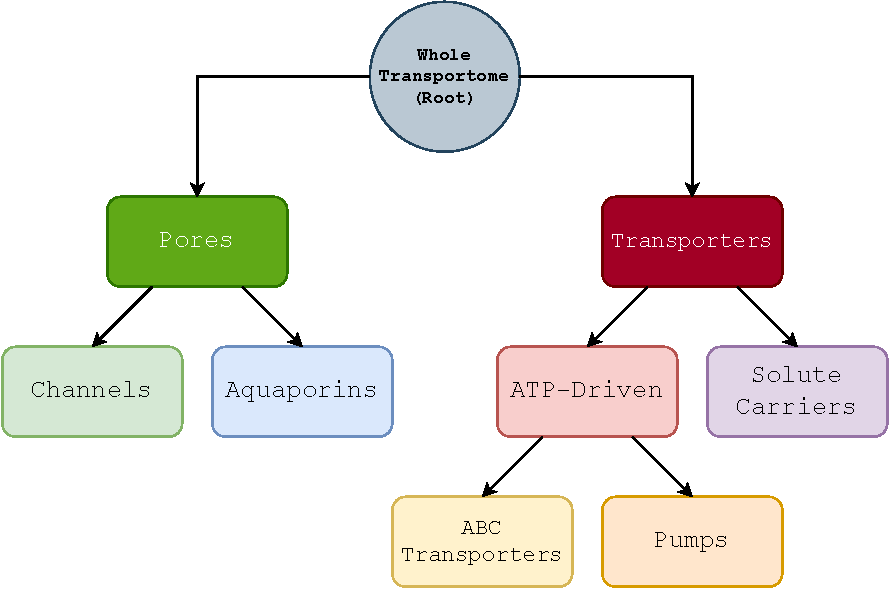
\includegraphics[width=0.65\textwidth]{resources/images/BasicTree.pdf}
    \caption{Minimal schema of the basic subdivisions of the Transportome genes used while generating \glspl{tgl}.}
    \label{fig:BasicTree}
\end{figure}

We created a Python script to query the database file produced by Daedalus and generate the the \glspl{tgl}. We structured the \glspl{tgl} as a directed acyclic graph, more specifically as a tree. In this tree, each node represents a separate \gls{tgl}: all transportome genes are present in the root node, while subsets of these gene sets are considered in every child node. This is very much alike the gene lists present in the \gls{go}.

To divide the genes into meaningful \glspl{tgl}, we seeded the algorithm to always produce a manually defined tree, or "core" tree, visible in Figure \ref{fig:BasicTree}. This subdivision purposefully follows the internal schema of the database: most nodes are represented by a table or a combination of whole tables. The algorithm then retrieves all available data for each node of the core tree, and finds all possible subdivisions of the original gene list based on the available data, appending each subdivision to the tree as a child node of the parent. This approach is then repeated for each added child, recursively creating smaller and smaller children gene sets.

In practice, for each "core" node, the database is queried to obtain the relevant (joined) columns of data available for the node. For instance, for the "ATP-Driven" core node, the algorithm will consider data from both the \mono{ABC\_transporters} and the \mono{atp\_driven\_transporters} tables. Once the data is retrieved from the database, for each available column the algorithm generates gene groups of unique genes with the same shared column value, appending them to the parent node. The algorithm then considers a subset of the original data, based on the column value used to generate the child gene set, and attempts to create more by considering all other columns in turn. This approach essentially enumerates all possible gene sets that could be meaningfully derived from the annotated data. 

This iterative process generates a very large number of gene sets. % Maybe specify how many?
For this reason, we implemented pruning on the resulting tree, which prunes away leaf nodes that are highly congruent with other nodes in the tree. For each leaf node $A$ in the tree $T$, containing a set of genes $A^g$, the algorithm computes the measure:
\begin{equation}
    \kappa = \max_{i:B_i \in T, B_i \ne A}\left(\frac{[(A^g - B_i^g) \cup (B_i^g - A^g)]}{[A^g \cap B_i^g]}\right)
    \label{eq:node_similarity}
\end{equation}
$\kappa$ is a value spanning from $0$ to $1$, where $1$ means perfectly congruent nodes, and $0$ meaning completely different nodes. If $\kappa$ is greater than an user-defined threshold value $\eta$ (generally close to 1), % MAYBE THIS IS WRONG? Generally close to 0?
the node is deemed redundant and pruned. When all leaves are considered, if the algorithm pruned at least one leaf, it is executed again. This process leaves a tree in which all leaf nodes are sufficiently different from each other. There might be congruence between internal nodes, but they cannot be eliminated without the removal of meaningful leaf nodes, so they are preserved.

% Lo so che e' una parculata - 'acute' - e la cambiamo, ma ci sta troppo bene
The acute reader might notice that this process removes leaves in an order-dependent way, as $\kappa$ is a symmetric measure, i.e. in Equation \ref{eq:node_similarity}, if the node $B_i$ causes the value of $\kappa$ for node $A$, then $A$ does the same to $B_i$. % This was (i.e $\kappa(A, B) = \kappa(B, A)$) but since the def of Kappa is over every other gene, it makes little sense. Might be better to rephrase the equation above.
This was taken into account, and the leaf nodes are sorted based on their depth (the number of edges to follow to return to the root node) before the pruning cycle begins. This allows the usage of two pruning strategies: bottom-up or top-down. In the top-down approach, higher leaves (farther from the root) are pruned first, as the nodes are sorted in descending order. The opposite happens in the bottom-up approach, where leaves closer to the root are pruned first, in favour of distant leaves.
% This might be a bit too much
Do note that although the measures are symmetrical, the two pruning methods do not generate trees that have an identical number of nodes: this is not surprising, as three nodes $A$, $B$ and $C$, where $\kappa(A) \because B > \eta$, $\kappa(B) \because C > \eta$ but $\kappa(A)  \because C < \eta$ will be pruned differently if they are considered in one order (e.g. $A \rightarrow B \rightarrow C$, resulting in $C$) than in another (e.g. $B \rightarrow C \rightarrow A$, resulting in $C, A$).

For efficiency purposes, the algorithm does not consider data columns that contain too many missing values (deeming them not meaningful to split on, with the default being $> 50\%$ emptiness), does not generate gene sets that are smaller than a threshold (by default $10$ genes) and does not consider for further subsetting gene sets smaller than a threshold (by default $40$).

It is important to note that the specifications for the "core" tree, the SQL calls used to retrieve the data for each node in the core tree, the threshold for $\kappa$, the pruning direction and other settings are all easily configurable in a separate file and/or as command-line arguments. This makes this approach easily adaptable to future versions of the \gls{mtpdb} and even other kinds of SQLite and more generally SQL-based databases provided by other researchers. The specification file used in our run is the default one (available on GitHub), and we used a $\kappa$ threshold of \todo{Set the treshold}.

Once generated, the tree is translated to a set of files in folders on disk. The folders are named with the names of the nodes, and the \mono{all.txt} files in them contain the Ensembl Gene IDs of the genes in the specific \gls{tgl}. This structure was chosen to easily allow the reconstruction of the tree by any other program, simply by following the tree-like file system paths.

\subsection{GSEA analysis}
Raw expression data data and metadata between \gls{tcga} and \gls{gtex} for this analysis was downloaded from the University of Santa Cruz's Xena platform \cite{UCSCXena}. Do note that TARGET samples were omitted from this analysis. This data has the benefit of being processed by the same analysis pipeline, eliminating technical noise coming from the pipeline itself. % If we run it barebones add version info. If we dockerize it, omit it.

To run \gls{gsea}, we needed to pair \gls{tcga} tumor expression data with their \gls{gtex} "healthy" counterparts and separately perform differential expression analysis on each cohort with the DESeq2 R package. This has proven not so simple a task. The Xena platform provides a fused version of the \gls{gtex} official metadata file plus the \gls{tcga} metadata for ease of use. However, it is unclear how to meaningfully pair such large databases, as methodology, possible batch effects due to sample handling, sample preprocessing (such as microdissection), and the intrinsic non-healthy nature of \gls{gtex} samples can cause confounding in the results. 

To pair the healthy and tumor data together, we followed the macroscopic grouping provided by the metadata files in the Xena platform. To subset the very large expression matrix file based on the metadata, we implemented a Python package called \mono{metasplit}. The specific calls used to subset the expression matrix and therefore match the tumor and healthy samples are \todo{AVAILABLE SOMEWHERE}. Generally, however, we compared tumor samples with their healthy counterparts from the same tissue or organ of origin.

% Is the following correct? -- We might want to talk about this later, or earlier.
This comparison is purposefully generic. As we lack specific information on the actual location of the biopsied tissue, its specific microdissection status, and potentially other experimental biases or variables at play, we deemed to be safer not to compare different tumor types of the same organ by themselves, but combine them into a more general category.

% We might want to discuss a bit about what the comparisons tell us, like we discussed internally.

The fitted DESeq2 model had only the tumor status variable and the intercept. This resulted in a t-statistic metric for each gene in each comparison. We ordered the gene lists according to this statistic, and used them to run a pre-ranked GSEA analysis with the fGSEA R package \cite{korotkevichFastGeneSet2021} using the previously generated genesets of interest.
We obtained one significance table for each tumor-healthy cohort, with enrichment information for each input gene set. We used this data to generate an enrichment matrix with the tree-like graph with the hierarchy of the genesets on the rows, the cohorts on the columns, and the \gls{nes} as values.

In order to see if independently-published dataset from single studies would compare with the results from the \gls{tcga}-\gls{gtex} analysis, we also gathered \todo{ADD NUMBER} independent datasets on \gls{pdac} samples from \gls{geo}, and subjected them to the same pipeline by comparing them to \gls{gtex} samples labelled as "Pancreas". The full table of dataset names and the studies they were sourced is available in Table \todo{ADD TABLE FROM GIORGIA}.

